\documentclass[11pt]{article}

\usepackage[a4paper,margin=1in]{geometry}
\usepackage[T1]{fontenc}
\usepackage[utf8]{inputenc}
\usepackage{lmodern}
\usepackage{amsmath}
\usepackage{graphicx}
\usepackage{caption}
\usepackage{booktabs}
\usepackage{hyperref}
\usepackage{pdfpages}

\renewcommand{\thefigure}{S\arabic{figure}}
\renewcommand{\thetable}{S\arabic{table}}

\begin{document}

\includepdf[pages=-,pagecommand={\thispagestyle{empty}}]{assets/supp_patched_intro_pages.pdf}
\includepdf[pages=3,pagecommand={\thispagestyle{empty}}]{../pyfgsea_supplementary.pdf}
\includepdf[pages=4,pagecommand={\thispagestyle{empty}}]{../pyfgsea_supplementary.pdf}
\includepdf[pages=5,pagecommand={\thispagestyle{empty}}]{../pyfgsea_supplementary.pdf}

\clearpage
\setcounter{page}{6}
\setcounter{figure}{6}
\setcounter{table}{3}

\begin{table}[htbp]
\centering
\caption{Runtime and peak memory usage comparison across implementations (example settings). All tools (including R/fgsea) were run with 4 threads.}
\label{tab:s4}
\begin{tabular}{llrrrr}
\toprule
Dataset & Metric & PyFgsea & GSEApy & BlitzGSEA & R fgsea \\
\midrule
Small (12k genes, 200 sets) & Time (s) & 0.16 & 5.06 & 5.22 & 6.37 \\
Small (12k genes, 200 sets) & RAM (MB) & 49.9 & 270.0 & 570.0 & 1309.3 \\
Medium (20k genes, 1k sets) & Time (s) & 0.35 & 22.57 & 7.06 & 5.62 \\
Medium (20k genes, 1k sets) & RAM (MB) & 53.7 & 1282.6 & 583.5 & 1414.5 \\
Large (20k genes, 5k sets) & Time (s) & 1.35 & 189.42 & 18.00 & 8.42 \\
Large (20k genes, 5k sets) & RAM (MB) & 68.0 & 5891.1 & 611.4 & 1620.0 \\
\bottomrule
\end{tabular}
\end{table}

\section*{S8. Core Mathematical Formulations and Multilevel Adaptive Sampling}

\begin{figure}[htbp]
\centering
\includegraphics[width=\textwidth]{assets/figure_S7_workflow.png}
\caption{Methodological workflow diagram. PyFgsea accepts ranked genes, a GMT collection, and multilevel estimation parameters as input; executes pathway-wise tasks in the Rust core using Rayon scheduling, deterministic per-pathway PRNG sub-seeds, Enrichment Score (ES) evaluation, and multilevel splitting logic; and finally aggregates ES/NES/$P$-value outputs across pathways and rolling windows.}
\label{fig:s7}
\end{figure}

\paragraph{Enrichment Score (ES) Calculation.}
For a ranked list of $N$ genes and a gene set $S$ of size $K$, the ES is defined as the maximum deviation from zero of a weighted random walk:
\[
ES = \max_{1 \le i \le N} \left( P_{\mathrm{hit}}(i) - P_{\mathrm{miss}}(i) \right).
\]
Using the standard weighted preranked GSEA notation, with ranked statistics $\{r_j\}_{j=1}^{N}$ and weight exponent $p$,
\[
P_{\mathrm{hit}}(i)=\sum_{\substack{j \le i \\ j \in S}} \frac{|r_j|^{p}}{\sum_{g \in S} |r_g|^{p}},
\qquad
P_{\mathrm{miss}}(i)=\sum_{\substack{j \le i \\ j \notin S}} \frac{1}{N-K}.
\]
Thus, $P_{\mathrm{hit}}(i)$ accumulates the normalized weighted contribution of genes in the pathway up to rank $i$, whereas $P_{\mathrm{miss}}(i)$ accumulates the complementary background walk over genes outside the pathway.

\paragraph{Random Pathway Generation.}
To build the background null distribution, PyFgsea generates random pathways by uniformly sampling $K$ genes without replacement from the given gene universe (all valid genes present in the input ranked list).

\paragraph{Multilevel Adaptive Sampling.}
The algorithm efficiently targets rare-event $P$-values by iterative splitting.

\paragraph{Initialization.}
An initial set of independent permutations ($N_{\mathrm{base}}$, e.g. 1000) is evaluated to form a baseline null distribution.

\paragraph{Iterative Splitting Rules.}
If the observed ES falls in the extreme tail, i.e. the estimated $P$-value approaches the resolution limit of the current sample size, the state space is split. Random walks that reach the current top threshold are cloned, and their remaining trajectories are simulated to conditionally explore rarer regions.

\paragraph{P-value Formula.}
The final tail probability is computed as the product of conditional probabilities across all $L$ splitting levels:
\[
P \approx P_0 \prod_{l=1}^{L} P\!\left(ES \ge c_l \mid ES \ge c_{l-1}\right).
\]

\paragraph{Stopping Conditions.}
Sampling recursively stops when the relative error (standard deviation) of the estimated $P$-value converges below a user-defined threshold, the computational budget is exhausted, or the calculated $P$-value drops below the absolute floor \texttt{eps} (e.g. $10^{-50}$).

\paragraph{Algorithm S1. Pseudocode-style summary of the PyFgsea multilevel routine.}
The following boxed summary is intended to make the current Rust implementation more directly auditable. It describes the release-\texttt{v0.1.4} multilevel workflow at a pseudocode level, while Table~\ref{tab:s5} separately clarifies which components are conceptually preserved from \texttt{fgseaMultilevel} and which are implementation-specific.

\begin{center}
\fbox{%
\begin{minipage}{0.95\textwidth}
\small
\textbf{Inputs:} ranked scores $\{r_j\}_{j=1}^{N}$, observed pathway hits $S$ with size $K$, observed metric $m_{\mathrm{obs}}$ derived from $ES_{\mathrm{obs}}$, baseline sample size $N_{\mathrm{base}}$, master seed, \texttt{eps}.\\[0.4em]
\textbf{Initialization:}
\begin{enumerate}
\item Draw $N_{\mathrm{base}}$ random size-matched pathways uniformly without replacement from the valid gene universe.
\item Compute each null-pathway ES and its tail metric $m_i$ using the same sign convention as the observed pathway.
\item Count $b_0=\#\{i: m_i \ge m_{\mathrm{obs}}\}$. If $b_0 \ge \lceil 0.05N_{\mathrm{base}}\rceil$, return the direct estimate $(b_0+1)/(N_{\mathrm{base}}+1)$.
\end{enumerate}
\textbf{Iterative multilevel splitting:}
\begin{enumerate}
\item At level $l$, set the current threshold $c_l$ to the empirical median of the population metric values, i.e. the cutoff at index $N_{\mathrm{base}}/2$ after partial sorting.
\item Let $b_l=\#\{i: m_i \ge m_{\mathrm{obs}}\}$. If $c_l \ge m_{\mathrm{obs}}$ or $b_l=N_{\mathrm{base}}$, stop and return $\exp(\log P_{l-1}) \times b_l/N_{\mathrm{base}}$.
\item Update the accumulated log-probability by the elite-survival factor, $\log P_l \leftarrow \log P_{l-1} + \log\!\left(\frac{N_{\mathrm{base}}/2}{N_{\mathrm{base}}}\right)$.
\item Retain the top half of the current population as elites.
\item For each non-elite slot, clone one elite pathway and rejuvenate it by a short constrained random walk of $w=\mathrm{clamp}(K,10,100)$ swap attempts:
\begin{enumerate}
\item remove one in-pathway gene and propose one out-of-pathway replacement;
\item recompute the candidate ES metric;
\item accept the proposal only if the candidate metric remains at least $c_l$; otherwise revert the swap.
\end{enumerate}
\item Record the acceptance rate for that level and continue to the next level until one of the stopping rules is met.
\end{enumerate}
\textbf{Finalization:} apply the absolute floor \texttt{eps}, return the estimated nominal $P$-value, and optionally expose level thresholds and acceptance rates for debugging.
\end{minipage}}
\end{center}

\section*{S9. Parallel Architecture and PRNG Management}

\paragraph{Task Allocation and Synchronization.}
Multi-threading is implemented via the Rust \texttt{rayon} crate utilizing a dynamic work-stealing thread pool. Parallelization is applied at the pathway level. Since evaluations for different pathways are conditionally independent given the pre-sorted ranked gene list, PyFgsea avoids complex cross-thread synchronization, data-merging locks, or mutexes, resulting in highly scalable execution.

\paragraph{Parallel Random Number Management.}
A critical challenge in parallel GSEA is ensuring exact statistical reproducibility. PyFgsea avoids a global shared random-state architecture. Instead, the user-provided master seed and the unique pathway string identifier (or index) are hashed together to generate a deterministic, independent sub-seed for each individual pathway. This sub-seed initializes a fast, thread-local PRNG stream. Consequently, under matched inputs and a fixed master seed, the stochastic simulation stream for any specific pathway remains strictly identical across runs despite changes in thread count or OS-level scheduling unpredictability.

\begin{table}[htbp]
\centering
\caption{Same-versus-different summary relative to the original fgseaMultilevel formulation.}
\label{tab:s5}
\resizebox{\textwidth}{!}{%
\begin{tabular}{p{0.18\textwidth}p{0.20\textwidth}p{0.21\textwidth}p{0.20\textwidth}p{0.17\textwidth}}
\toprule
Component & Preserved from fgseaMultilevel & Implementation-level difference in PyFgsea & Functional extension in PyFgsea & Expected impact on outputs \\
\midrule
ES definition & Same weighted preranked ES statistic and signed random-walk target & Implemented in Rust/PyO3 rather than the R execution stack & None & ES values remain numerically identical within machine precision under matched inputs \\
Null-pathway generation & Same size-matched random pathway sampling from the valid ranked-gene universe & Deterministic pathway-local sub-seeds are derived from the master seed and pathway identifier & None & Null sampling stays statistically aligned while becoming thread-count invariant \\
Multilevel tail factorization & Same product-of-conditional-probabilities rare-event estimator & Tail levels are executed in a compiled backend with lightweight object marshalling & None & Deep-tail behaviour follows the same estimator family while improving throughput \\
Level construction & Same progressively conditioned rare-event levels & Current Rust release realizes levels through empirical median thresholding plus elite-clone rejuvenation under deterministic pathway-local PRNG streams (Algorithm S1) & None & Makes the implemented level schedule explicit while preserving the same rare-event target \\
Precision policy & Same multilevel sampling logic and stopping interpretation & PyFgsea exposes a stricter default floor (\texttt{eps=1e-50}) than the historical R default (\texttt{eps=1e-10}) & None & Outputs match in the common range; PyFgsea can additionally report rarer tails at finer resolution \\
Parallel execution model & Same pathway-wise conditional independence assumption exploited for acceleration & Rayon dynamic work stealing replaces R-side scheduling and avoids cross-thread locks & None & Output values are preserved while runtime scales with thread count under fixed seeds \\
Trajectory workflow & Same preranked per-window GSEA logic once a ranked vector is formed & Stateful runner reuses pathway definitions and NES background structures across windows & Rolling-window trajectory analysis for pseudotime-ordered single-cell data & Functional scope extends beyond the original single ranked-list workflow without altering per-window GSEA semantics \\
\bottomrule
\end{tabular}
}
\end{table}

\section*{S10. Rolling-Window Boundary Handling and Sensitivity}

\paragraph{Parameter Sensitivity Analysis (Figure~\ref{fig:s8}).}
Figure~\ref{fig:s8} now summarizes both window-size and step-size sensitivity across three representative pathways (heme metabolism, E2F targets, and G2-M checkpoint). Small windows exhibit high sensitivity to localized expression changes but are more vulnerable to single-cell technical noise, causing jagged and statistically unstable NES fluctuations. Conversely, overly large windows behave as low-pass filters, oversmoothing the trajectory and potentially masking rapid biological transitions. Step size mainly controls the density of pathway sampling along pseudotime and the computational footprint: coarse steps preserve broad trends but can skip narrow transient peaks, whereas finer steps provide denser temporal localization at higher computational cost.

\paragraph{Guidelines.}
A practical starting range is a window size covering roughly 5--10\% of total cells with a step size near 1--2\% of total cells, but this should be tuned to trajectory length and noise level. Step size linearly dictates the computational footprint and temporal granularity. The illustrative erythroid case study in the main text intentionally uses a slightly larger 500-cell baseline window (approximately 14\% of that trajectory) because the analyzed lineage segment is relatively short and noisy, and the figure prioritizes a smoother reference profile over maximal temporal resolution. The current erythroid sensitivity grid brackets rather than directly centers this generic starting range, spanning approximately 2.8\%, 14.0\%, and 28.0\% of cells for the tested windows. At the trajectory end, the default production workflow avoids padding-induced edge artifacts by stopping at the last full window; Section~S13 below additionally audits a separate explicit terminal-truncation extension.

\begin{figure}[htbp]
\centering
\includegraphics[width=0.95\textwidth]{assets/figure_S8_window_sensitivity.png}
\caption{Rolling-window parameter sensitivity across three representative Hallmark pathways in the real erythroid trajectory analysis. Left column: varying window size (100, 500, 1000 cells) at fixed step size 50. Right column: varying step size (20, 50, 100 cells) at fixed window size 500. Smaller windows capture transient local structure but amplify noise, whereas larger windows smooth the curves; coarser step sizes reduce temporal sampling density and can miss short-lived NES peaks.}
\label{fig:s8}
\end{figure}

\begin{table}[htbp]
\centering
\caption{Compact quantitative summary of agreement with the R reference used to complement the main-text statistics. Log$_{10}P$ refers to transformed nominal $P$-values, i.e. $-\log_{10}(P)$.}
\label{tab:s6}
\begin{tabular}{lrrrr}
\toprule
Metric & Pearson $r$ & Spearman $\rho$ & RMSE & Median $|\Delta|$ \\
\midrule
NES (PyFgsea vs R) & 1.000 & 1.000 & 0.0135 & 0.0070 \\
ES (PyFgsea vs R) & 1.000 & 1.000 & 0.0000 & 0.0000 \\
Log$_{10}P$ (PyFgsea vs R) & 0.997 & 0.988 & 0.1696 & 0.0467 \\
\bottomrule
\end{tabular}
\end{table}

\section*{S11. Comprehensive Validation and Reproducibility Assessment of PyFgsea}

This section provides an integrated validation of PyFgsea across numerical equivalence, stochastic stability, and reproducibility under repeated and parallel execution. The goal is not to repeat the methodological details already summarized in Sections~S8--S10, but to make the implementation claims directly testable through a compact, reviewer-oriented validation package.

\begin{figure}[htbp]
\centering
\includegraphics[width=\textwidth]{assets/figure_S9_validation_overview.png}
\caption{End-to-end validation overview map. The new validation package is organized around four complementary axes: statistical faithfulness to the R \texttt{fgseaMultilevel} reference, deterministic reproducibility under repeated and parallel execution, pathway-level scalability of the parallel backend, and robustness of rolling-window trajectory analysis under parameter and boundary stress tests.}
\label{fig:s9}
\end{figure}

\paragraph{S11.1 Validation design and benchmark regimes.}
To make the revised supplement more self-contained, we validated PyFgsea across both synthetic and trajectory-derived ranked lists. The synthetic regimes span small, medium, and large benchmark sizes. The trajectory-derived regimes reuse the erythroid case study from the main text, but extract representative early, middle, and late ranked windows directly from the pseudotime ordering before running standard preranked GSEA against the same Hallmark collection. Across all regimes, pathway size filters, \texttt{sampleSize}, and \texttt{eps} were harmonized between PyFgsea and R/\texttt{fgseaMultilevel}.

\paragraph{S11.2 Integrated ES/NES/$P$-value equivalence.}
Figure~\ref{fig:s10} consolidates equivalence evidence across all benchmark regimes and across three output levels: ES, NES, and transformed nominal $P$-values. ES remained numerically identical within machine precision in every regime. NES concordance remained uniformly very high (all Pearson $r>0.9999$), whereas transformed nominal $P$-values were slightly more dispersed in sparse local trajectory windows, as expected for adaptive rare-event estimation on noisier local rank statistics. The weakest transformed nominal-$P$ concordance occurred in the early trajectory window (Table~\ref{tab:s7}), where only 43 Hallmark pathways passed the size filter and several strongly enriched programs occupied a locally sensitive tail regime. In that setting, moderate absolute nominal-$P$ differences are amplified by the $-\log_{10}(P)$ transform, even though ES remained identical within machine precision and NES stayed near-identical. Accordingly, ES and NES are the more robust primary cross-implementation comparanda in sparse local windows, whereas transformed nominal-$P$ agreement is more sensitive to tail-estimation noise and pathway-count filtering.

\begin{figure}[htbp]
\centering
\includegraphics[width=\textwidth]{assets/figure_S10_equivalence_overview.png}
\caption{Integrated equivalence validation across synthetic benchmarks and representative trajectory windows. Each panel aggregates pathway-wise outputs from six regimes (three synthetic benchmark sizes plus early, middle, and late erythroid trajectory windows) and compares PyFgsea against the R \texttt{fgseaMultilevel} reference for (A) ES, (B) NES, and (C) transformed nominal $P$-values. Colors indicate benchmark regime; dashed lines indicate identity.}
\label{fig:s10}
\end{figure}

\begin{table}[htbp]
\centering
\caption{Quantitative equivalence summary across all validation regimes. The expanded table complements the concise main-text metrics by reporting ES, NES, and transformed nominal $P$-value concordance separately for each synthetic benchmark and each representative erythroid trajectory window.}
\label{tab:s7}
\scriptsize
\resizebox{\textwidth}{!}{\begin{tabular}{llrrrrr}
\toprule
Regime & Metric & Pearson $r$ & Spearman $\rho$ & RMSE & Median $|\Delta|$ & 95th pct. $|\Delta|$ \\
\midrule
Synthetic small & ES & 1.000 & 1.000 & 0.0000 & 0.0000 & 0.0000 \\
Synthetic small & NES & 1.000 & 1.000 & 0.0178 & 0.0072 & 0.0342 \\
Synthetic small & Log10P & 0.997 & 0.994 & 0.1536 & 0.0360 & 0.4010 \\
Synthetic medium & ES & 1.000 & 1.000 & 0.0000 & 0.0000 & 0.0000 \\
Synthetic medium & NES & 1.000 & 0.999 & 0.0155 & 0.0095 & 0.0268 \\
Synthetic medium & Log10P & 0.997 & 0.989 & 0.0941 & 0.0344 & 0.2025 \\
Synthetic large & ES & 1.000 & 1.000 & 0.0000 & 0.0000 & 0.0000 \\
Synthetic large & NES & 1.000 & 0.999 & 0.0145 & 0.0102 & 0.0282 \\
Synthetic large & Log10P & 0.992 & 0.986 & 0.1072 & 0.0301 & 0.2213 \\
Trajectory early & ES & 1.000 & 1.000 & 0.0000 & 0.0000 & 0.0000 \\
Trajectory early & NES & 1.000 & 0.998 & 0.0135 & 0.0080 & 0.0262 \\
Trajectory early & Log10P & 0.941 & 0.976 & 0.3286 & 0.0693 & 0.8734 \\
Trajectory middle & ES & 1.000 & 1.000 & 0.0000 & 0.0000 & 0.0000 \\
Trajectory middle & NES & 1.000 & 0.999 & 0.0163 & 0.0104 & 0.0346 \\
Trajectory middle & Log10P & 0.990 & 0.940 & 0.2045 & 0.0721 & 0.3980 \\
Trajectory late & ES & 1.000 & 1.000 & 0.0000 & 0.0000 & 0.0000 \\
Trajectory late & NES & 1.000 & 0.997 & 0.0141 & 0.0103 & 0.0255 \\
Trajectory late & Log10P & 0.996 & 0.972 & 0.1880 & 0.0737 & 0.4999 \\
\bottomrule
\end{tabular}
}
\end{table}

\paragraph{S11.3 Cross-thread determinism under a fixed master seed.}
Because pathway-level reproducibility under parallel execution is central to the implementation claim, we explicitly audited fixed-seed thread-count invariance before turning to repeated-run stability. Figure~\ref{fig:s11} shows that pathway-wise outputs and pathway ranking remained invariant across thread counts in this benchmark, directly supporting the deterministic pathway-local PRNG strategy described in Section~S9.

\begin{figure}[htbp]
\centering
\includegraphics[width=\textwidth]{assets/figure_S11_thread_validation.png}
\caption{Cross-thread determinism and scaling under a fixed master seed. (A) Pathway-level execution shows near-linear speedup at lower thread counts with modest memory variation. (B) Deterministic sub-seeding guarantees identical pathway-wise outputs and identical pathway ranking across thread counts in this audit.}
\label{fig:s11}
\end{figure}

\paragraph{S11.4 Fixed-seed reproducibility versus multi-seed variability.}
Repeated executions should be interpreted in two distinct ways. Under a fixed input and a fixed master seed, the implementation should be deterministic. Under changing seeds, modest variability in multilevel tail estimates is expected because the rare-event estimator remains stochastic. Figure~\ref{fig:s12} explicitly separates these two regimes. The left panel collapses to nearly degenerate distributions under a fixed seed, whereas the right panel shows the bounded stochastic envelope obtained when varying seeds over repeated runs.

\begin{figure}[htbp]
\centering
\includegraphics[width=\textwidth]{assets/figure_S12_reproducibility.png}
\caption{Run-to-run reproducibility audit. Under a fixed seed (left), repeated executions are effectively identical, confirming deterministic end-to-end behaviour. Under varying seeds (right), pathway-level $-\log_{10}(P)$ values fluctuate within a modest stochastic envelope, reflecting the expected Monte Carlo variability of adaptive multilevel sampling rather than implementation instability.}
\label{fig:s12}
\end{figure}

\section*{S12. Parallel Execution Validation and Scalability Audit}

\paragraph{S12.1 Thread-count invariance under deterministic pathway-local PRNG streams.}
Section~S9 described the design principle: pathway evaluations are conditionally independent and therefore scheduled in parallel, while each pathway receives a deterministic sub-seed derived from the user-provided master seed and pathway identifier. Figure~\ref{fig:s11} and Table~\ref{tab:s8} convert that design claim into an explicit audit. Across thread counts from 1 to 16, pathway-wise outputs remained exactly invariant under a fixed seed, with exact-match and identical-ranking fractions equal to 1.000 throughout this benchmark.

\begin{table}[htbp]
\centering
\caption{Parallel reproducibility audit across thread counts. Exact-match and identical-ranking fractions were computed relative to the 1-thread reference under the same input data and the same master seed.}
\label{tab:s8}
\scriptsize
\resizebox{\textwidth}{!}{\begin{tabular}{rrrrrrrr}
\toprule
Threads & Time (s) & Speedup & Peak RSS (MB) & Exact match & Rank match & Max $|\Delta NES|$ & Max $|\Delta -\log_{10}P|$ \\
\midrule
1 & 0.691 & 1.00 & 6.4 & 1.000 & 1.000 & 0.0e+00 & 0.0e+00 \\
2 & 0.369 & 1.87 & 3.5 & 1.000 & 1.000 & 0.0e+00 & 0.0e+00 \\
4 & 0.221 & 3.13 & 7.4 & 1.000 & 1.000 & 0.0e+00 & 0.0e+00 \\
8 & 0.149 & 4.64 & 9.7 & 1.000 & 1.000 & 0.0e+00 & 0.0e+00 \\
16 & 0.119 & 5.80 & 4.8 & 1.000 & 1.000 & 0.0e+00 & 0.0e+00 \\
\bottomrule
\end{tabular}
}
\end{table}

\paragraph{S12.2 Stateful versus stateless rolling-window execution.}
To isolate the practical benefit of the stateful runner used in trajectory analysis, we benchmarked repeated trajectory-derived score vectors against a 3000-pathway stress-test collection. As shown in Figure~\ref{fig:s15}, reusing pathway definitions and NES background structures yielded a consistent end-to-end wall-time advantage over repeatedly calling stateless preranked GSEA. The gain was stable across 100, 300, and 1000 windows (roughly 1.9-fold in this conservative end-to-end stress test), demonstrating that the rolling-window runner reduces repeated overhead without changing the per-window statistical target. This value should be interpreted alongside the larger 7.47-fold speedup reported in the original Supplementary Table~S3: that earlier number came from a narrower 100-window component benchmark with 5000 pathways and therefore emphasized amortized preprocessing and NES-background reuse more strongly. We therefore report the conservative end-to-end figure first and interpret the larger number as a scope-specific component benchmark rather than a universal whole-workflow gain.

\section*{S13. Rolling-Window Robustness and Parameter Stress Tests}

\paragraph{S13.1 Window-size and step-size stress test.}
The original sensitivity addition in Figure~\ref{fig:s8} already demonstrated that both window size and step size influence the shape of NES trajectories for three representative pathways. Here we summarize the same grid more explicitly in a reviewer-oriented form. Figure~\ref{fig:s13} converts the full $3\times3$ window-by-step grid into compact summaries of smoothness, peak-position drift, significant-window overlap, and runtime. Smaller windows increased temporal responsiveness but amplified stepwise NES roughness and reduced agreement with the baseline setting; coarse step sizes reduced runtime but also reduced significant-window overlap by undersampling local transients.

\begin{figure}[htbp]
\centering
\includegraphics[width=\textwidth]{assets/figure_S13_parameter_grid_summary.png}
\caption{Rolling-window parameter stress-test summary over the full window-size by step-size grid. Heatmaps summarize four practical readouts averaged across three representative pathways: stepwise NES roughness, peak-position shift relative to the baseline setting (window 500, step 50), significant-window overlap, and runtime.}
\label{fig:s13}
\end{figure}

\begin{table}[htbp]
\centering
\caption{Rolling-window parameter sensitivity summary across the full grid. The table reports the effective window/step percentages relative to the erythroid trajectory, the number of windows, average smoothness and peak-shift diagnostics, significant-window overlap relative to the baseline setting (window 500, step 50), and measured runtime.}
\label{tab:s9}
\scriptsize
\resizebox{\textwidth}{!}{\begin{tabular}{rrrrrrrrr}
\toprule
Window & Step & Window (\%) & Step (\%) & Windows & Median stepwise $|\Delta NES|$ & Peak-shift & Sig. overlap & Runtime (s) \\
\midrule
100 & 20 & 2.8 & 0.6 & 174 & 0.1858 & 0.0210 & 0.477 & 7.6 \\
100 & 50 & 2.8 & 1.4 & 70 & 0.2792 & 0.0130 & 0.435 & 3.0 \\
100 & 100 & 2.8 & 2.8 & 35 & 0.4780 & 0.0152 & 0.384 & 1.6 \\
500 & 20 & 14.0 & 0.6 & 154 & 0.0627 & 0.0083 & 0.608 & 7.9 \\
500 & 50 & 14.0 & 1.4 & 62 & 0.1273 & 0.0000 & 1.000 & 3.2 \\
500 & 100 & 14.0 & 2.8 & 31 & 0.2423 & 0.0576 & 0.692 & 1.6 \\
1000 & 20 & 28.0 & 0.6 & 129 & 0.0490 & 0.0841 & 0.483 & 7.3 \\
1000 & 50 & 28.0 & 1.4 & 52 & 0.1054 & 0.0854 & 0.387 & 2.9 \\
1000 & 100 & 28.0 & 2.8 & 26 & 0.2166 & 0.0857 & 0.323 & 1.4 \\
\bottomrule
\end{tabular}
}
\end{table}

\paragraph{S13.2 Boundary-handling audit at trajectory termini.}
Reviewer 2 also asked for clearer boundary handling. To make the edge behaviour more transparent, Figure~\ref{fig:s14} now separates the audit into three complementary views: the changing cell count of terminal windows, representative pathway trajectories, and a pathway-level continuity summary relative to the last full window. The main-text Figure~2 uses the default full-window workflow only, whereas the audit here evaluates a separate terminal-truncation extension that adds progressively smaller tail windows without any padding. The resulting NES trajectories continue smoothly rather than showing abrupt edge artifacts. Quantitatively, the truncation-only tail windows retain high pathway-level agreement with the last full window, supporting the use of non-padded terminal handling while making the end-of-trajectory behaviour visually explicit.

\begin{figure}[htbp]
\centering
\includegraphics[width=\textwidth]{assets/figure_S14_boundary_audit.png}
\caption{Boundary-handling audit near the trajectory terminus. (A) Audit design: terminal truncation progressively shortens tail windows beyond the last full 500-cell window instead of padding the trajectory end. (B--C) Representative pathway trajectories showing that the truncation extension continues the local NES trend smoothly for heme metabolism and E2F targets. (D) Quantitative continuity summary for truncation-only tail windows relative to the last full window, reported as pathway-level Spearman correlation of NES values and top-10 pathway overlap.}
\label{fig:s14}
\end{figure}

\begin{figure}[htbp]
\centering
\includegraphics[width=\textwidth]{assets/figure_S15_stateful_scaling.png}
\caption{Stateful versus stateless rolling-window scaling on trajectory-derived score vectors under a 3000-pathway stress test. Reusing cached pathway definitions and NES background structures yields a consistent end-to-end wall-time advantage as the number of windows increases.}
\label{fig:s15}
\end{figure}

\paragraph{S13.3 Practical parameter guidance.}
Taken together, Figures~\ref{fig:s8}, \ref{fig:s13}, and \ref{fig:s14} support the empirical guidance used in the revised main text. For exploratory scans, window sizes near 5--10\% of cells with step sizes near 1--2\% of cells provide a practical starting range, but the setting should still be tuned to trajectory length, local noise, and the desired degree of smoothing. The current erythroid grid brackets rather than directly centers this generic range. The 500-cell baseline used for the erythroid illustration is deliberately somewhat larger than this starting range because that lineage segment is comparatively short and noisy; in practice, larger windows are appropriate when the goal is a smoother descriptive profile rather than fine transition localization. Smaller windows should be interpreted as high-resolution but noise-sensitive views, whereas larger windows behave more like smoothed summaries of broad trajectory trends.

\section*{S14. Summary of Validated Claims and Practical Guidance}

The revised supplement now closes the loop between algorithm description and observable software behaviour. Table~\ref{tab:s10} maps each major manuscript claim to the concrete experiment, metric, and empirical conclusion supporting it.

\begin{table}[htbp]
\centering
\caption{Validated-claims summary linking manuscript claims to the new supplementary validation package.}
\label{tab:s10}
\resizebox{\textwidth}{!}{%
\begin{tabular}{p{0.24\textwidth}p{0.20\textwidth}p{0.18\textwidth}p{0.28\textwidth}} 
\toprule
Manuscript claim & Validation experiment & Metric(s) & Result and reference \\
\midrule
PyFgsea remains statistically aligned with \texttt{fgseaMultilevel} & Integrated cross-regime equivalence audit & ES/NES/$-\log_{10}(P)$ concordance & ES was identical within machine precision; NES remained uniformly near-identical; transformed nominal $P$-values were highly concordant overall (Figure~\ref{fig:s10}, Tables~\ref{tab:s6} and \ref{tab:s7}) \\
Parallel execution is reproducible under a fixed master seed & Cross-thread determinism audit from 1 to 16 threads & Exact-match fraction, identical-ranking fraction, max absolute differences & All audited thread counts yielded exact pathway-wise matches and identical pathway ranking in this benchmark (Figure~\ref{fig:s11}, Table~\ref{tab:s8}) \\
Repeated runs separate implementation stability from expected Monte Carlo variability & Fixed-seed and varying-seed repeated executions & Distribution of pathway-wise $-\log_{10}(P)$ over repeated runs & Fixed-seed reruns collapsed to effectively identical outputs, whereas changing seeds produced only bounded stochastic tail variation (Figure~\ref{fig:s12}) \\
Rolling-window conclusions are robust but parameter-dependent & Multi-pathway window/step stress test plus terminal boundary audit & NES roughness, peak shift, significant-window overlap, runtime & Smaller windows and coarser steps trade stability for resolution and runtime; baseline settings preserved the best overlap while terminal handling remained smooth and non-padded (Figures~\ref{fig:s8}, \ref{fig:s13}, and \ref{fig:s14}; Table~\ref{tab:s9}) \\
The stateful trajectory runner reduces repeated computational overhead & Stateful-versus-stateless trajectory stress test & End-to-end wall-time speedup & A conservative 3000-pathway end-to-end stress test showed an approximately 1.9-fold wall-time advantage, consistent with the larger 7.47-fold gain reported in the narrower 100-window component benchmark of the original Supplementary Table~S3 (Figure~\ref{fig:s15}) \\
\bottomrule
\end{tabular}}
\end{table}

\section*{S15. Limitation Audit of the Rolling-Window Ranking Statistic}

The revised Discussion now explicitly acknowledges two practical limitations of the rolling-window ranking statistic used in trajectory analysis: (i) genes or pathways with complex non-monotonic dynamics may be underestimated, increasing false-negative risk; and (ii) sparse, high-variance genes may be over-amplified, creating local false-positive peaks. To make these caveats directly observable rather than merely verbal, we added the targeted audit below. The goal is not to defend the statistic as universally optimal, but to show where it behaves stably, where it begins to fail, and how simple sensitivity checks can help users interpret local pathway peaks more cautiously.

\paragraph{S15.1 Real-data examples of how the limitation manifests.}
Figure~\ref{fig:s16} uses four representative genes from the real erythroid pseudotime analysis to visualize the relationship between smoothed single-gene expression, the actual rolling-window ranking signal used by the method, and a related Hallmark pathway NES trajectory. Monotonic programs (for example, HBB or IFI27) produce ranking traces that remain easy to interpret. In contrast, transient or non-monotonic genes (for example, MKI67 and JUNB) generate ranking traces that are broader, more asymmetric, or more locally mixed than the underlying smoothed expression profile, illustrating why temporally localized biology can be blurred or phase-shifted by the window-versus-rest statistic. Because the released erythroid matrix is a dense standardized layer rather than a raw-count matrix with preserved dropout structure, the sparse/high-variance failure mode is audited below through semi-simulation rather than by raw-gene plots alone.

\begin{figure}[htbp]
\centering
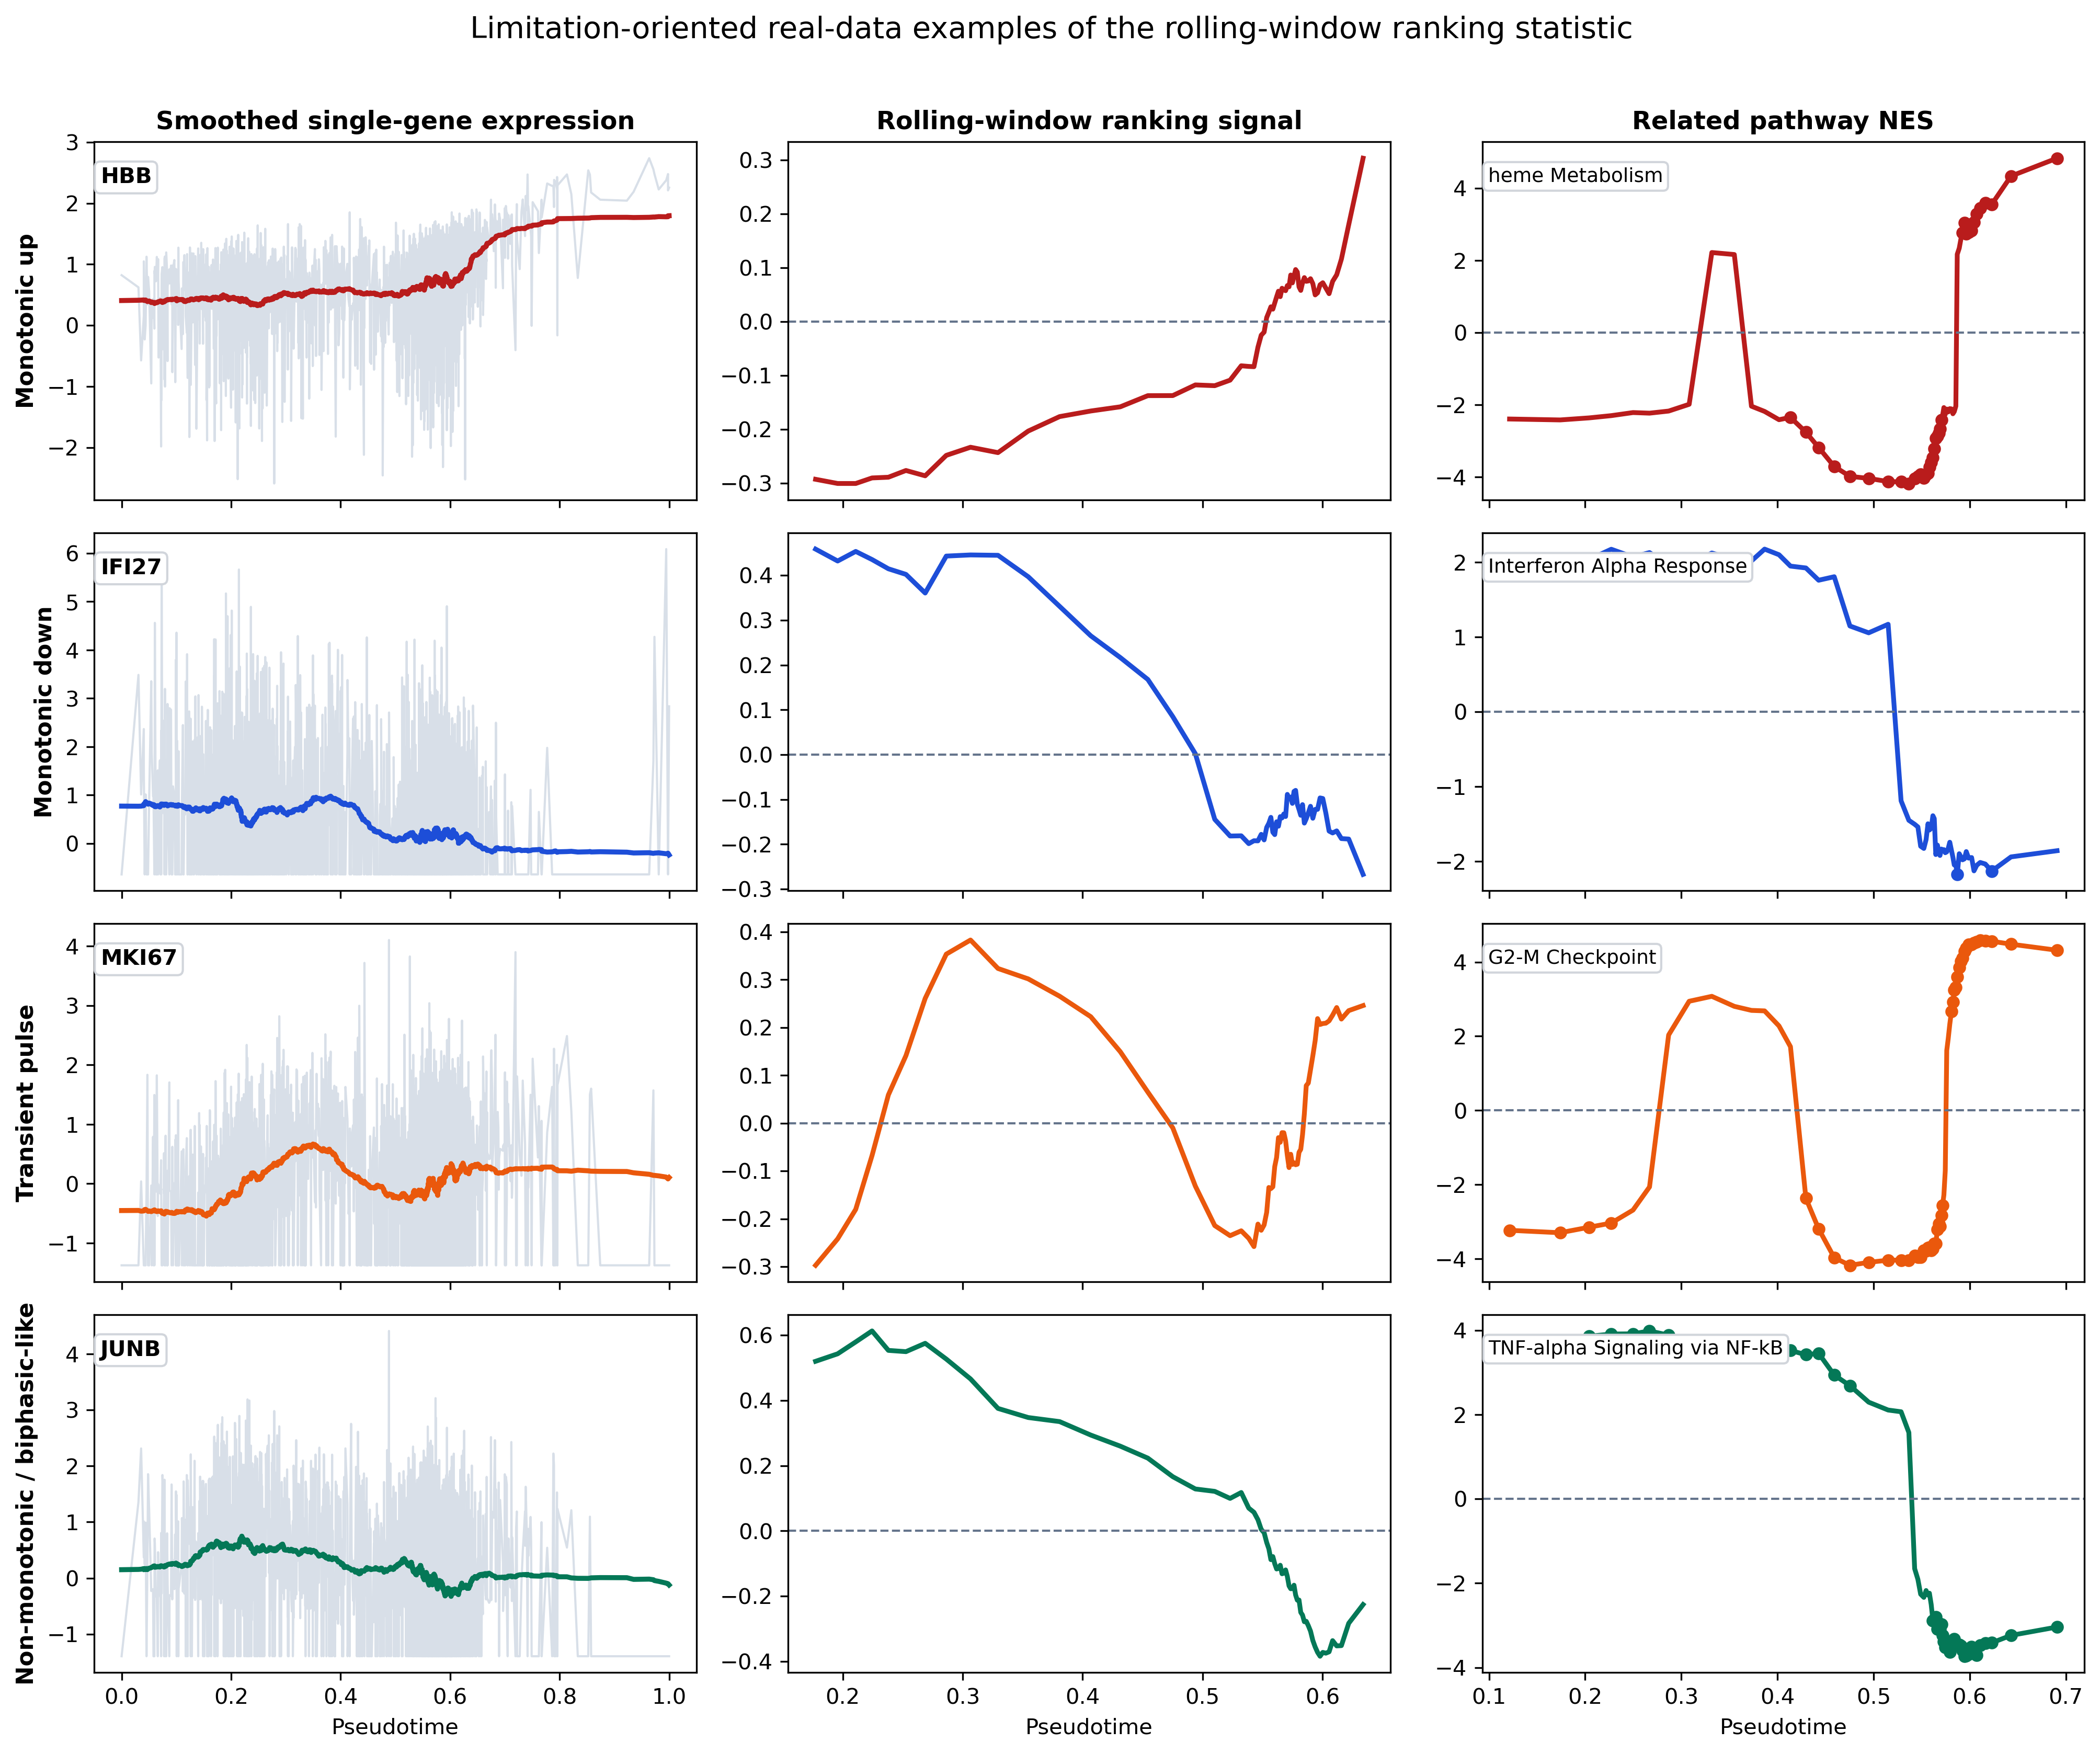
\includegraphics[width=\textwidth]{assets/figure_S16_limitation_examples.png}
\caption{Real-data limitation-oriented examples from the erythroid trajectory. Each row shows (left) the smoothed single-gene expression profile, (middle) the corresponding rolling-window ranking signal used by the method, and (right) a related Hallmark pathway NES curve under the same rolling-window settings. Monotonic genes produce comparatively stable ranking traces, whereas transient or non-monotonic genes generate broader or locally mixed ranking signals, illustrating the mechanism underlying potential false-negative pathway calls for complex temporal programs.}
\label{fig:s16}
\end{figure}

\paragraph{S15.2 Semi-simulated audit of false-negative and false-positive regimes.}
To test these limitations more directly, we embedded synthetic pathway genes into the real erythroid pseudotime cell ordering while keeping a large background of real standardized genes. Four pathway archetypes were examined: a coherent monotonic program, a narrow transient pulse, a mixed biphasic program consisting of early- and late-peaking subgroups, and a sparse high-variance burst process with no latent biological trajectory. Figure~\ref{fig:s17} overlays the latent pathway signal with the observed NES trajectories returned by the current rolling-window statistic. The monotonic pathway remained the most stable reference case. The transient pathway remained detectable but its peak shifted slightly earlier than the latent optimum. The mixed biphasic pathway showed a markedly smaller number of significant windows despite matched per-gene amplitude, because early and late subprograms diluted each other within the same pathway. Finally, the sparse-noise pathway had a flat latent truth yet still produced localized positive NES peaks, directly illustrating the false-positive mechanism discussed in the revised main-text Discussion.

\begin{figure}[htbp]
\centering
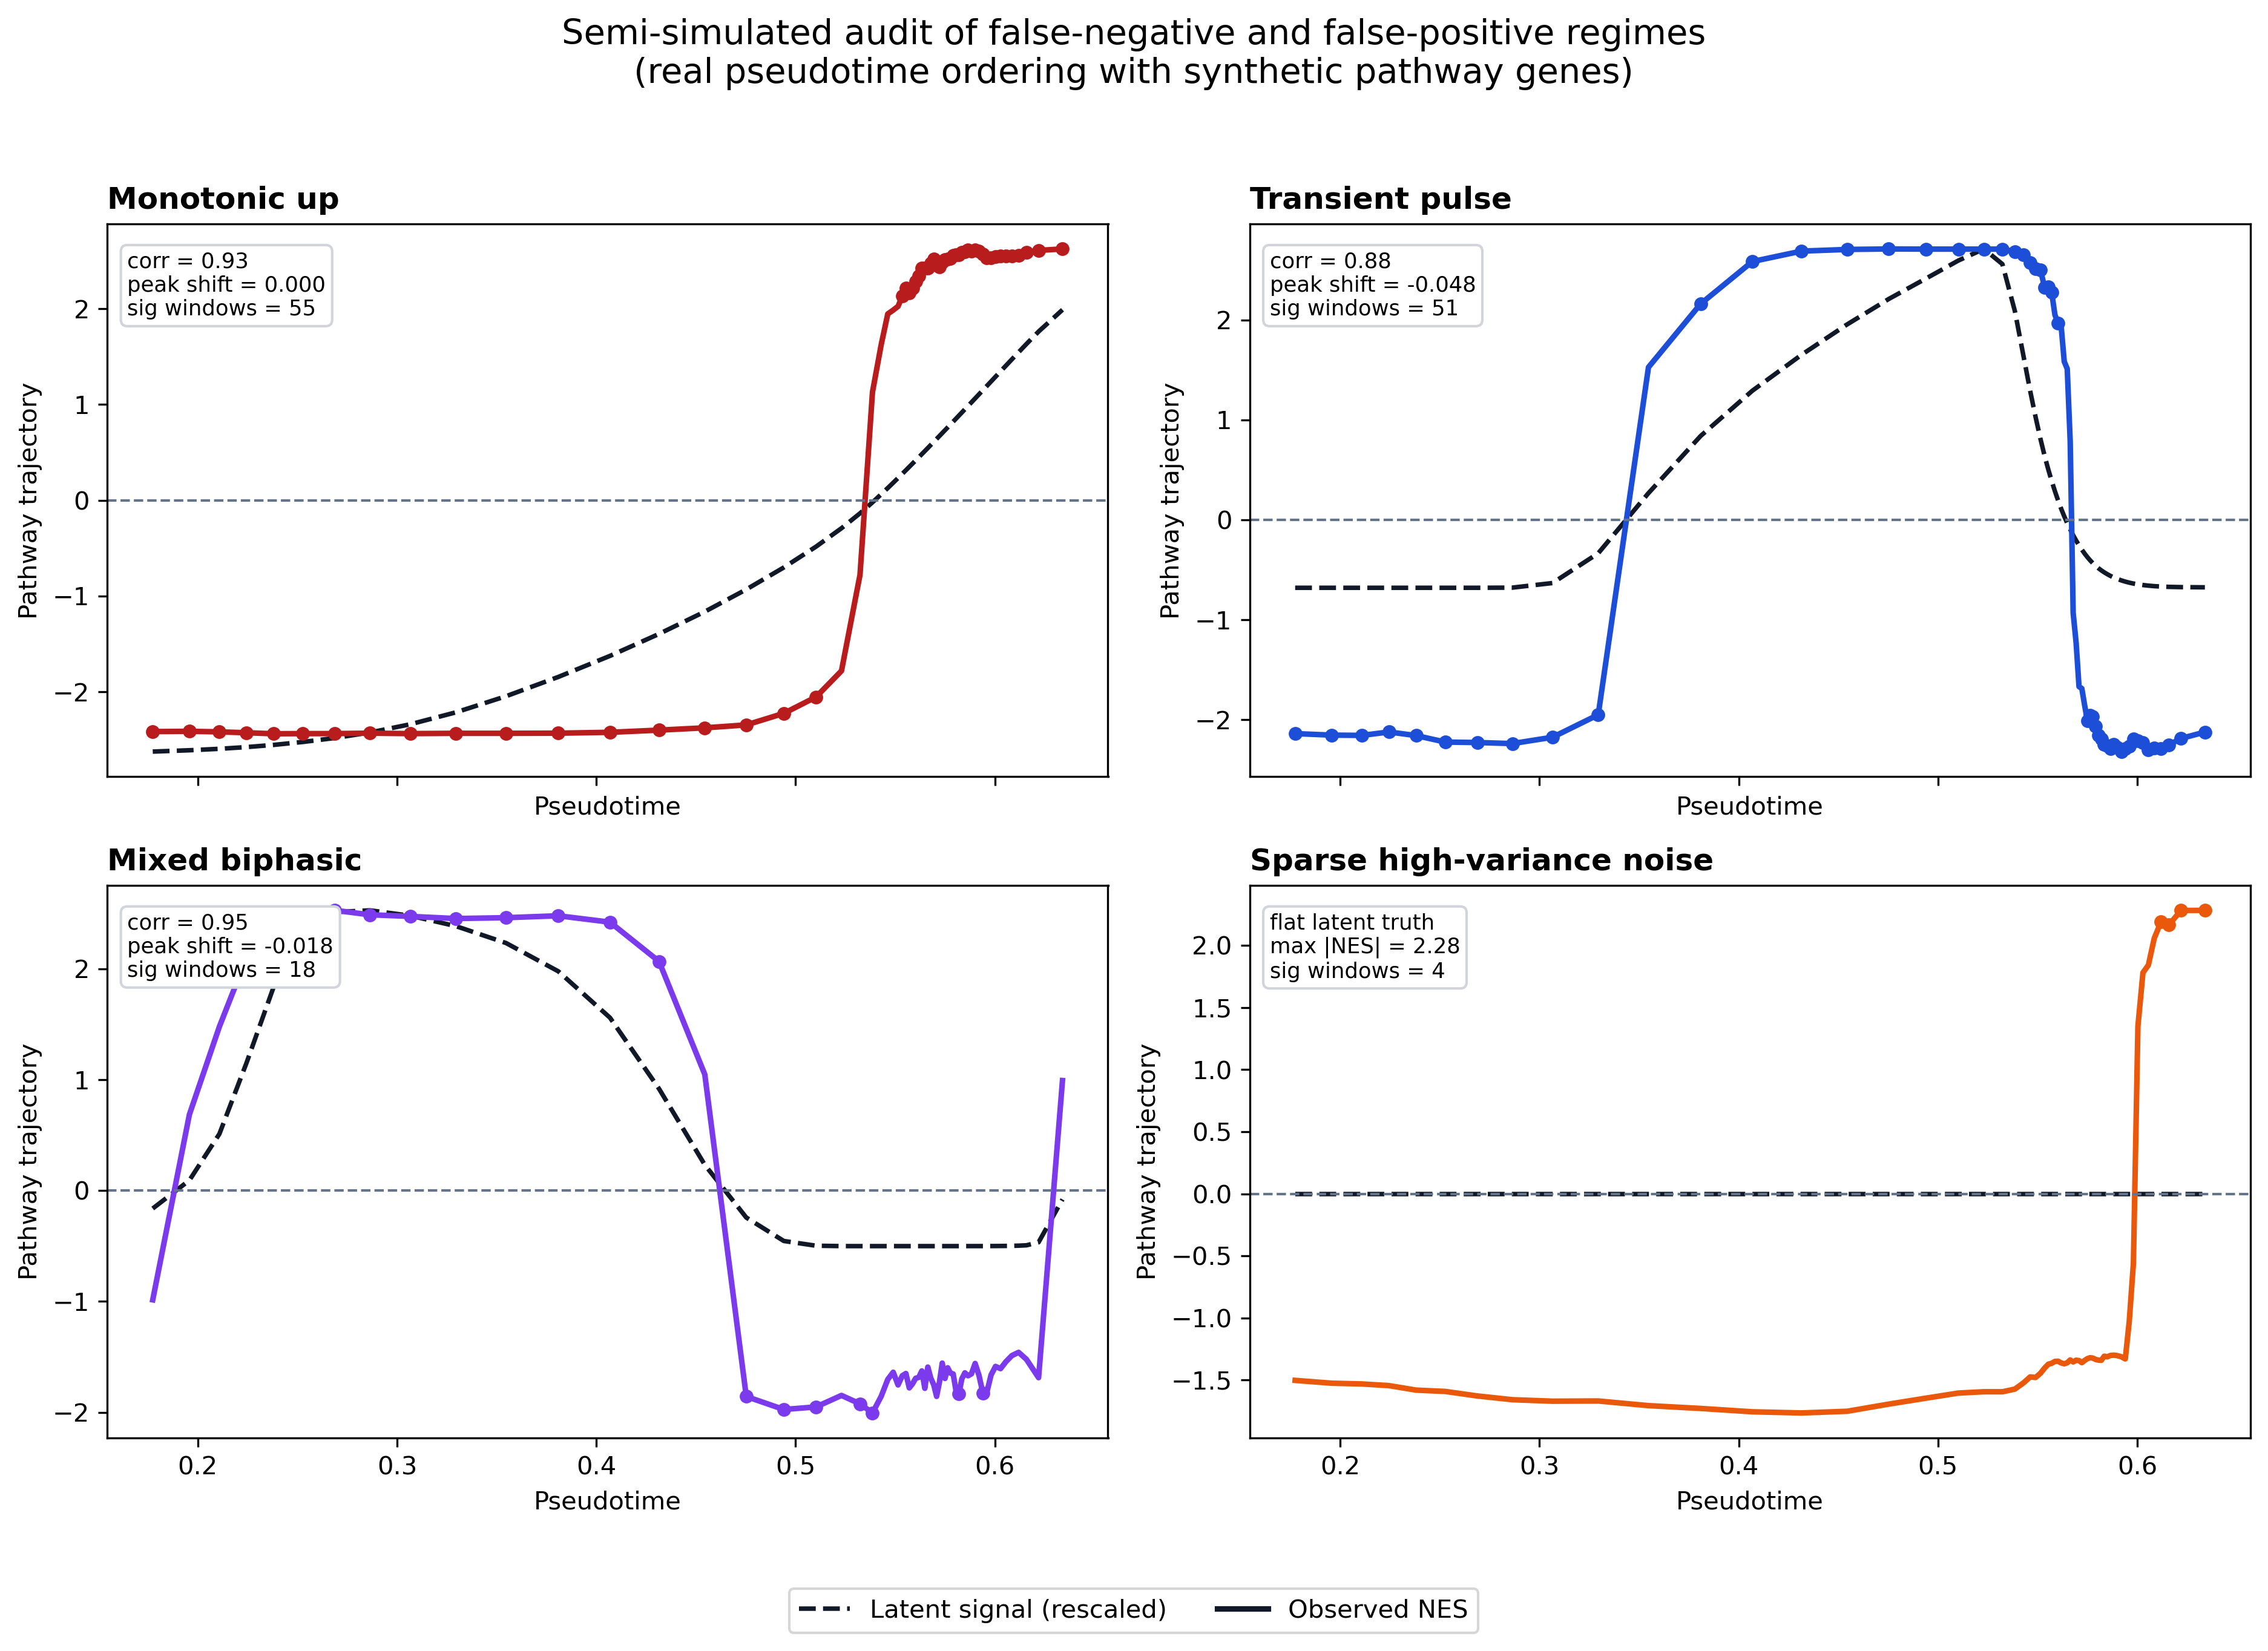
\includegraphics[width=\textwidth]{assets/figure_S17_limitation_benchmark.png}
\caption{Semi-simulated limitation audit on the real erythroid pseudotime ordering. Dashed curves show the latent pathway signal (rescaled for visual comparison), whereas colored curves show the observed NES trajectories returned by the current rolling-window statistic. The monotonic pathway behaves stably; the narrow transient pulse is shifted slightly; the mixed biphasic pathway is attenuated and yields fewer significant windows; and the sparse high-variance pathway shows local positive NES peaks despite a flat latent truth.}
\label{fig:s17}
\end{figure}

\paragraph{S15.3 Sensitivity-check control for sparse/high-variance pathways.}
We did not replace the main ranking statistic in the revised manuscript. However, as a sensitivity check, Figure~\ref{fig:s18} compares the current trajectory workflow against a simple detection-rate-weighted control that downweights genes observed in only a tiny fraction of cells. This control is not proposed as the new default method; it is included only to test whether the sparse/high-variance failure mode is real. The result is informative: monotonic and transient pathways change very little, whereas the sparse-noise pathway loses its false-positive windows under the weighted control. This reinforces the interpretation that extreme local peaks should be cross-checked when they are driven by very low-detection genes.

\begin{figure}[htbp]
\centering
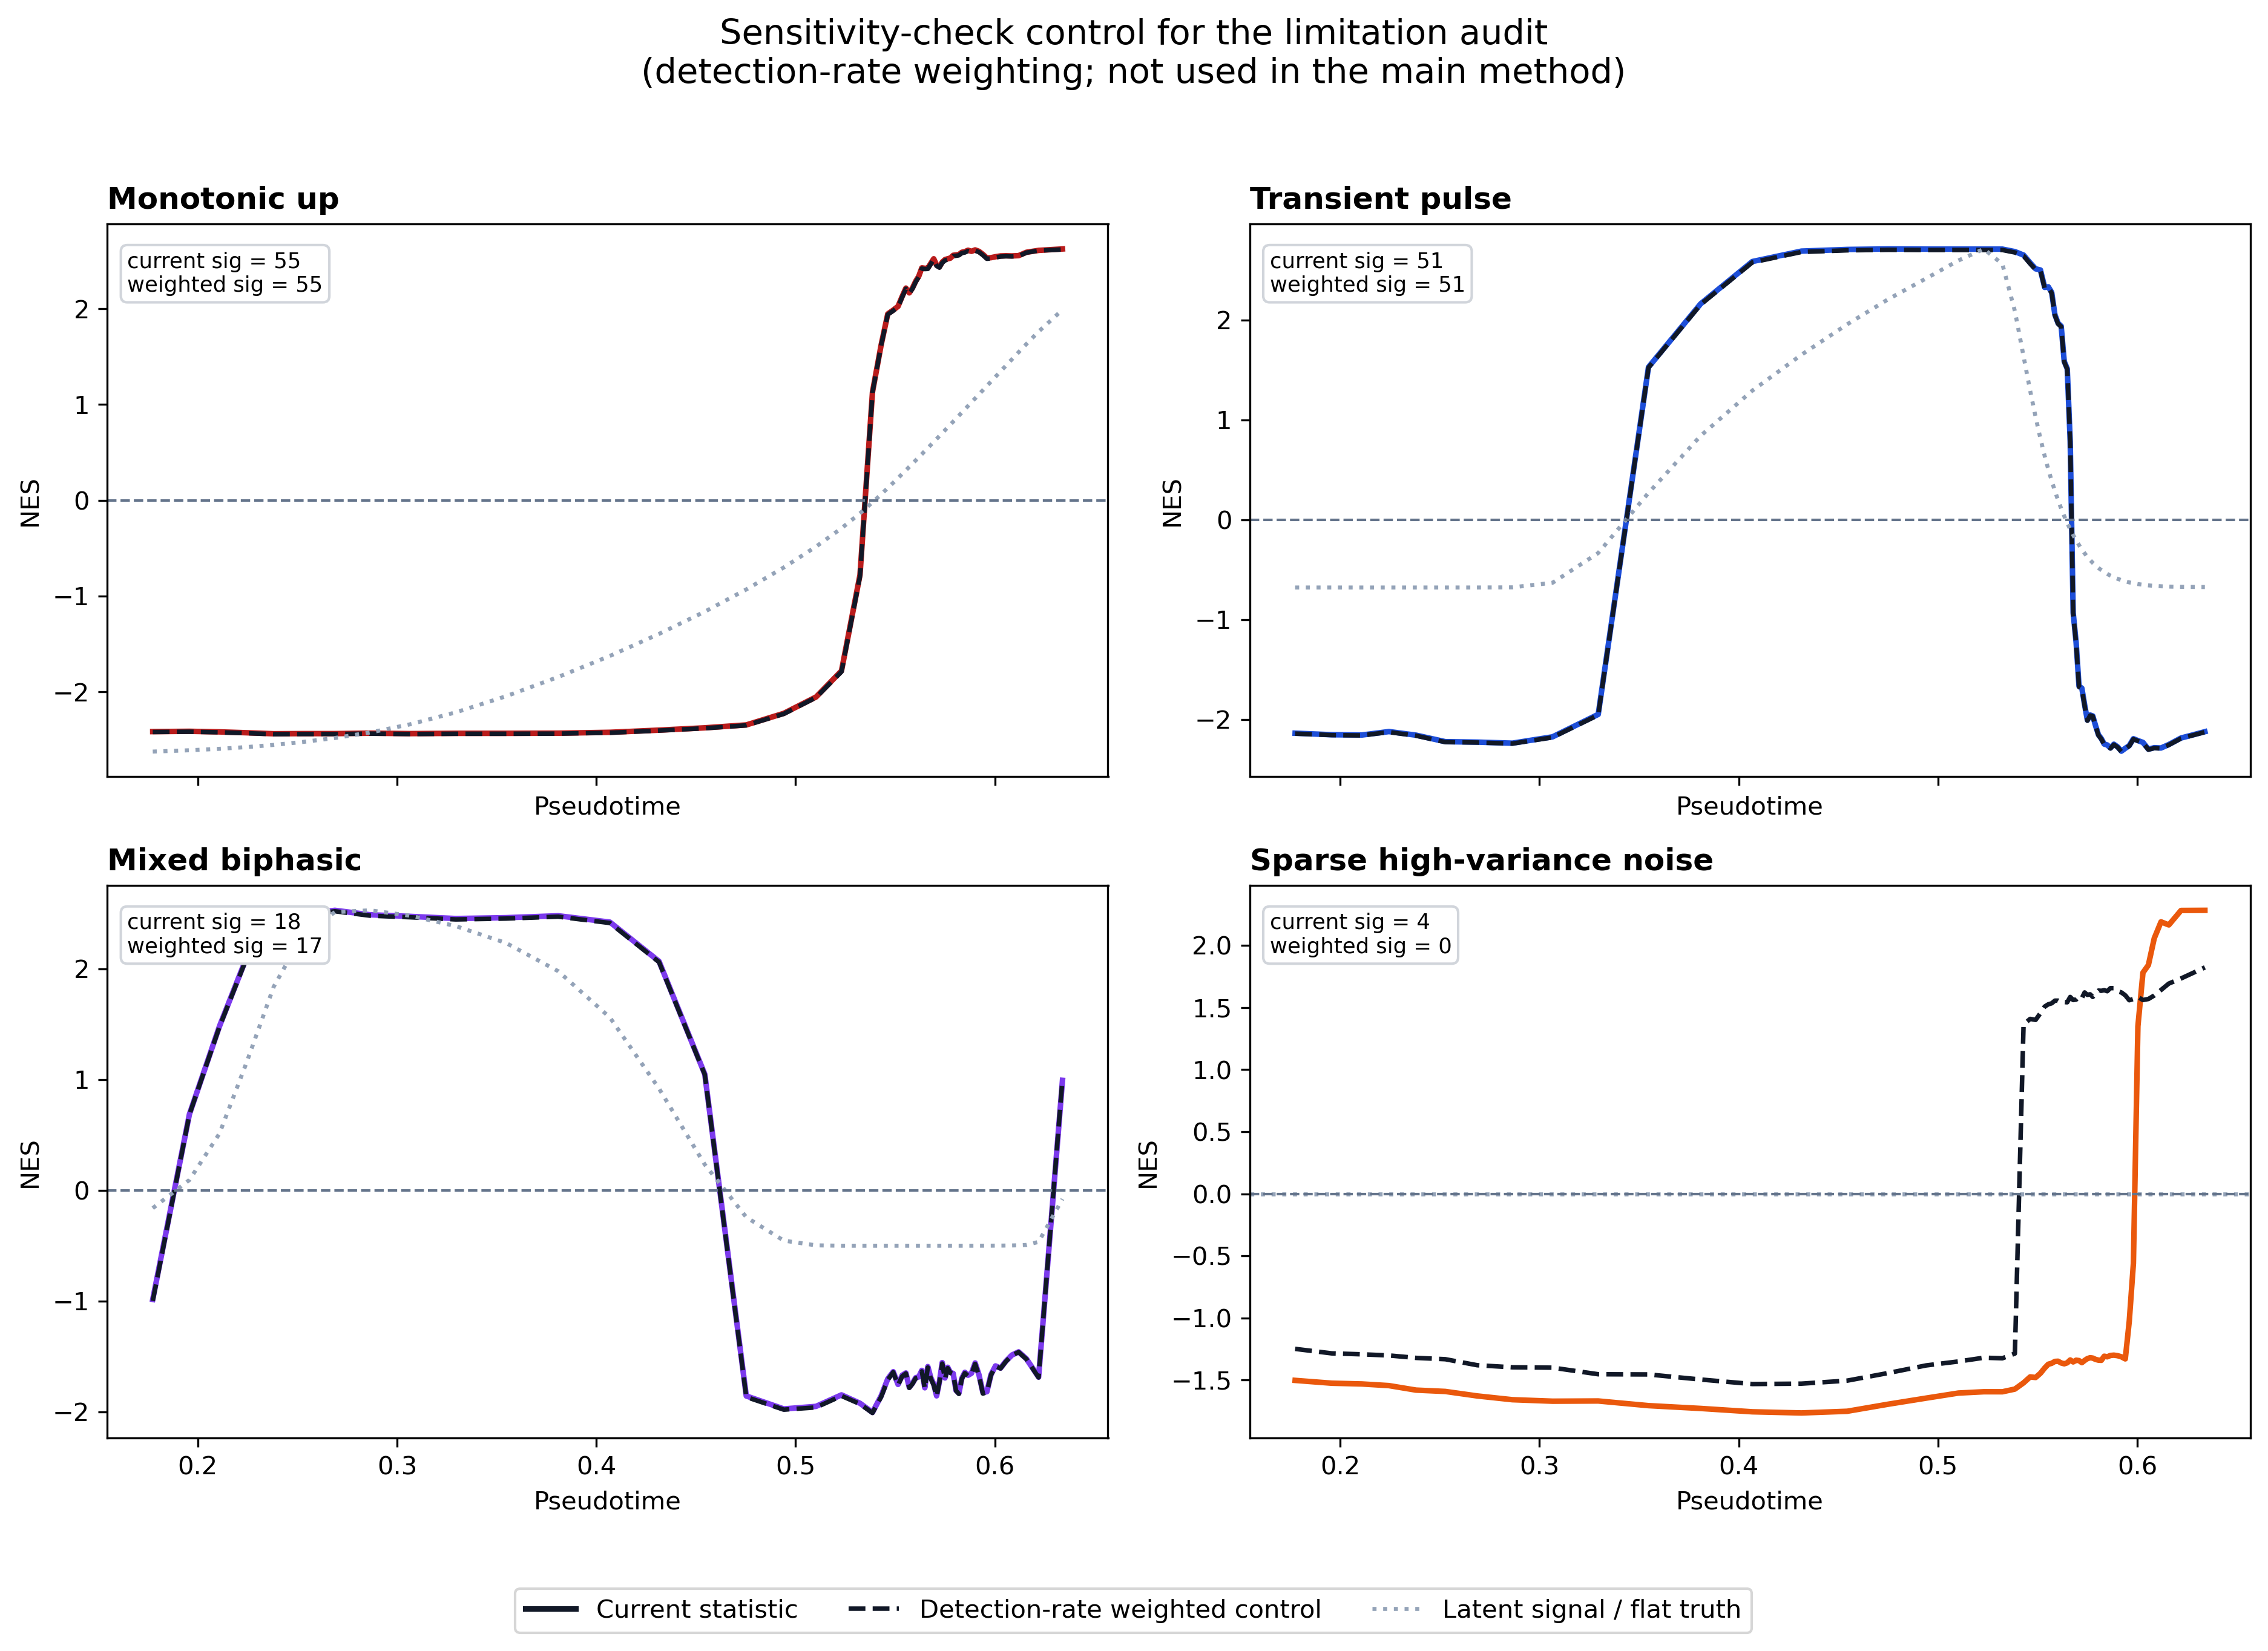
\includegraphics[width=\textwidth]{assets/figure_S18_limitation_control.png}
\caption{Sensitivity-check control for the limitation audit. Solid lines show the current rolling-window statistic, dashed black lines show a simple detection-rate-weighted control, and dotted gray lines show the latent pathway signal or flat latent truth. The control barely changes the monotonic baseline but attenuates the sparse-noise pathway enough to remove its significant windows, supporting the interpretation that low-detection, high-variance genes can drive local false-positive enrichments.}
\label{fig:s18}
\end{figure}

\begin{table}[htbp]
\centering
\caption{Compact summary of the limitation-oriented audit. Corr.\ denotes the correlation between the latent pathway signal and the observed NES trajectory in the semi-simulation; peak shift is reported in pseudotime units. The detection-rate-weighted control is included as a sensitivity check only and is not the primary method used in the main manuscript.}
\label{tab:s11}
\scriptsize
\resizebox{\textwidth}{!}{\begin{tabular}{p{0.17\textwidth}p{0.10\textwidth}p{0.11\textwidth}p{0.10\textwidth}p{0.10\textwidth}p{0.11\textwidth}p{0.25\textwidth}}
\toprule
Pattern & Corr. (current) & Peak shift & Sig. windows & Weighted sig. & Max $|NES|$ (cur$\rightarrow$wt) & Interpretation \\
\midrule
Monotonic up & 0.93 & 0.000 & 55 & 55 & 2.63$\rightarrow$2.62 & Monotonic pathway behaviour remained stable and served as the baseline reference. \\
Transient pulse & 0.88 & -0.048 & 51 & 51 & 2.71$\rightarrow$2.70 & The narrow pulse remained detectable but its peak shifted slightly earlier than the latent optimum. \\
Mixed biphasic & 0.95 & -0.018 & 18 & 17 & 2.53$\rightarrow$2.52 & Early and late subprograms diluted each other, reducing the number of significant windows despite matched per-gene amplitude. \\
Sparse high-variance noise & -- & -- & 4 & 0 & 2.28$\rightarrow$1.82 & Sparse high-variance bursts generated local false-positive windows; a simple detection-rate-weighted control attenuated them. \\
\bottomrule
\end{tabular}
}
\end{table}

\end{document}
